
\section{Methodology}
\label{sec:methodology}

Achieving the detailed goals requires the following research strategy:

\begin{enumerate}[label=\alph*)]
  \item To perform an exhaustive review of the state of the art in the areas 
  of user, context and device modelling, semantic reasoning and ontologies.   
  This analysis has been reinforced by attending specialized scientific   
  congresses.
  
  \item Perform a critical evaluation of the existing solutions, analysing 
  their limitations and scope and identifying the corresponding areas where it 
  was possible to make a contribution to the state of the art.
  
  \item To design and develop the different modules of AdaptUI infrastructure, 
  by gradually extending their scope and capabilities.
  
  \item To carry out several experiments and evaluate the performance of the 
  developed modules.
  
  \item Attending congresses to present the achieved contributions with the 
  purpose of receiving the corresponding feedback from the scientific 
  community.
  
  \item Network with experts at conferences and meetings.
  
  \item Update the contributions and redesign the system with the feedback 
  attained from the previous actions.
  
  \item To develop and deploy the final dynamic user interface adaptation 
  infrastructure, which takes into account the user, context and device current 
  characteristics to provide the best suitable user interface.
  
  \item Disseminate the results obtained to the scientific community.
\end{enumerate}

Figure~\ref{fig:methodology} summarizes and illustrated the cited and 
followed methodology.


\begin{figure}[H]
\centering
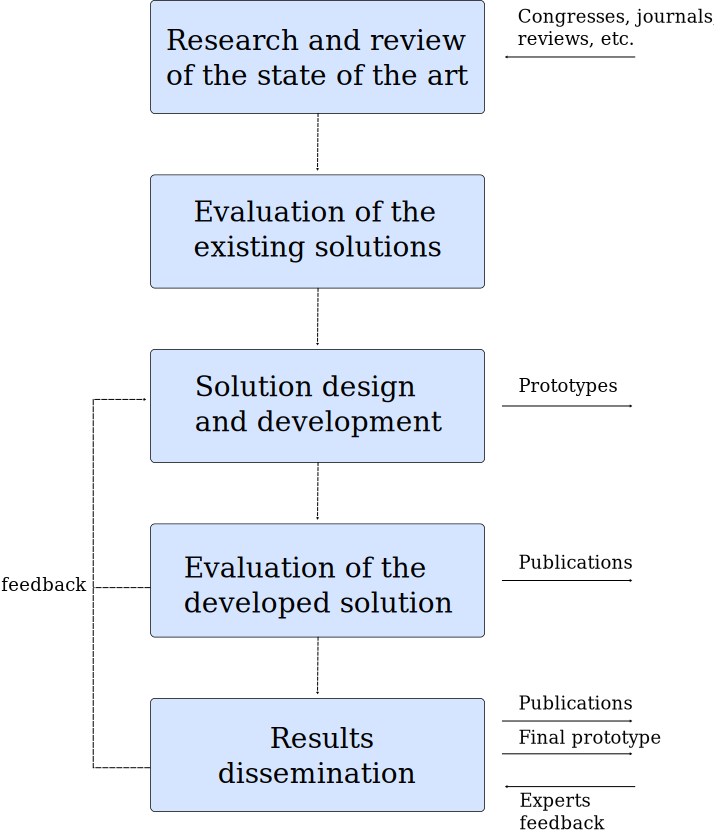
\includegraphics[width=0.60\textwidth]{methodology.pdf}
\caption{Followed research methodology.}
\label{fig:methodology}
\end{figure}